% Printable study notes for Semester Test 2 (COS711 Assignment 1).
% Build:  cd docs && tectonic test-notes.tex
\documentclass[11pt,a4paper]{article}
\usepackage[margin=2cm,headheight=14pt]{geometry}
\usepackage[T1]{fontenc}
\usepackage{lmodern}
\usepackage{microtype}
\usepackage{graphicx}
\usepackage{float}
\usepackage{booktabs}
\usepackage{tabularx}
\usepackage{xltabular}
\usepackage{array}
\usepackage{amsmath}
\usepackage{amssymb}
\usepackage{enumitem}
\usepackage[font=small,labelfont=bf]{caption}
\usepackage[hidelinks]{hyperref}
\usepackage{titlesec}
\usepackage{fancyhdr}
\usepackage{tikz}
\usepackage[most]{tcolorbox}

\graphicspath{{../figures/report/}}
\setlist{itemsep=2pt,topsep=3pt,leftmargin=*}
\setlength{\parskip}{0.45em}
\setlength{\parindent}{0pt}
\renewcommand{\arraystretch}{1.2}
\newcolumntype{Y}{>{\raggedright\arraybackslash}X}

\newcommand{\A}{\,\text{\AA}}
\newcommand{\verdict}[1]{\fbox{\footnotesize\textbf{#1}}}

% Running header: the section name, so you can flip to the right part quickly.
\pagestyle{fancy}
\fancyhf{}
\fancyhead[L]{\small\textsc{COS711 A1 test notes}}
\fancyhead[R]{\small\leftmark}
\fancyfoot[C]{\small\thepage}
\renewcommand{\sectionmark}[1]{\markboth{\thesection\quad #1}{}}

\titleformat{\section}{\Large\bfseries}{\thesection}{0.6em}{}
\titleformat{\subsection}{\large\bfseries}{\thesubsection}{0.5em}{}
\titleformat{\subsubsection}{\normalsize\bfseries}{\thesubsubsection}{0.5em}{}
\titlespacing*{\section}{0pt}{1.2em}{0.6em}
\titlespacing*{\subsection}{0pt}{1em}{0.4em}

% Boxes
\newtcolorbox{cheat}[2][]{breakable, enhanced, colback=black!4, colframe=black!75,
  fonttitle=\bfseries, title={#2}, boxrule=0.8pt, arc=1mm, left=2mm, right=2mm, #1}
\newtcolorbox{keyidea}[1][Key idea]{breakable, enhanced, colback=white, colframe=black!45,
  fonttitle=\bfseries\small, coltitle=black, colbacktitle=black!10, title={#1},
  boxrule=0.5pt, arc=1mm, left=2mm, right=2mm}

% Questions: numbered across the whole document so they are easy to refer to.
\newcounter{qnum}
\newcommand{\Q}[1]{\refstepcounter{qnum}\par\medskip\noindent\textbf{Q\theqnum.\ #1}\par\nopagebreak\noindent\ignorespaces}

\begin{document}

% ---------------------------------------------------------------- title page
\begin{center}
{\LARGE\bfseries COS711 Assignment 1: Test Notes}\\[0.4em]
{\large MLP on Protein Tertiary Structure: data preparation, core investigation, warmup and pruning}\\[0.3em]
{\small Kyle Liebenberg \quad u22608789 \quad Semester Test 2}
\end{center}

\begin{keyidea}[How to use these notes]
\begin{itemize}
  \item Every section explains the \emph{idea} first, then what \emph{we} did, then what happened and \emph{why}.
  \item Every section ends with a \textbf{cheat sheet} (the short version) and \textbf{likely questions} with
        answers. The questions are phrased generically, because the test has to work for all five datasets.
  \item Section~\ref{sec:generic} is a bank of general research-method questions, and Section~\ref{sec:glossary}
        is a glossary for quick look-ups.
  \item Units: RMSD and RMSE are in \textbf{ångström (\AA)}. Lower RMSE is better. ``Accuracy'' in the spec means
        our error metric, because our task is regression.
\end{itemize}
\end{keyidea}

\begin{keyidea}[The answer template: use it for any ``experiment'' question]
\textbf{1. Hypothesis} (what we predicted, and the theory behind it) $\;\to\;$
\textbf{2. Design} (what we changed, what we held fixed, how we measured) $\;\to\;$
\textbf{3. Result} (the key numbers) $\;\to\;$
\textbf{4. Verdict} (supported / partly / contradicted) $\;\to\;$
\textbf{5. Why} (connect the result back to theory; if we were wrong, say what our reasoning missed).
\end{keyidea}

\tableofcontents
\newpage

% ================================================================ 0
\section{The whole project on one page}
\label{sec:overview}

\subsection*{The task}
In the CASP protein-folding competition, scientists measure a protein's true 3D shape and keep it secret.
Prediction programs then produce many \textbf{candidate shapes (``decoys'')} for that protein. Each row of our
dataset is one decoy, described by \textbf{9 physicochemical measurements (F1--F9)}, such as surface areas and
how much water-repelling surface is exposed. The target is the decoy's \textbf{RMSD}: how far its atoms are from the
true shape, in ångström. 0 means perfect, around 2 means very close, and around 15 means essentially wrong.

Our MLP takes the measurements in and predicts the RMSD out. That makes it a \textbf{regression} task. It is useful
because for a new protein the true shape is unknown, so a model like this can rank thousands of candidates and point
to the likely best ones.

\subsection*{What the spec asked, and what we did}
\begin{tabularx}{\linewidth}{@{}p{3.3cm}YY@{}}
\toprule
Part & Spec asks & We did \\
\midrule
Data preparation & Feature relevance, outliers, scaling, splitting, imbalance & Removed duplicates, dropped F2, log + clip, z-score, stratified 80/20 split with 5-fold CV, per-bin evaluation \\
Core investigation & A baseline, then $\geq 2$ axes with k-fold CV, a hypothesis before each & Baseline 2$\times$64 MLP, then 3 axes: \textbf{optimisers, architecture, activation functions} \\
Research investigation & Warmup vs no warmup at comparable accuracy, magnitude pruning, identical fine-tuning, $\geq 3$ seeds, interpret the mechanism & Conditions A, B, C; global magnitude pruning at 0--98\%; 5 seeds; extensions E1, E2, E3 \\
\bottomrule
\end{tabularx}

\subsection*{The numbers worth remembering}
\begin{tabularx}{\linewidth}{@{}lY@{}}
\toprule
Rows & 45{,}730 raw $\to$ \textbf{44{,}019} after removing 1{,}711 exact duplicates \\
Split & \textbf{35{,}215 train / 8{,}804 test} (80/20), stratified on 3\A{} RMSD bins, seed 42 \\
Inputs & \textbf{8} features (F2 dropped because F2 = F1 $\times$ F3 exactly) \\
Baseline & 2$\times$64 ReLU MLP, Adam $10^{-3}$: CV RMSE \textbf{4.09\A}, $R^2 = 0.555$ \\
Reference models & Predict the mean 6.14\A; linear regression 5.19\A; gradient-boosted trees 4.13\A \\
Best model & 4$\times$256 ReLU, Adam $10^{-3}$: CV \textbf{3.81\A}; test \textbf{3.78 $\pm$ 0.03\A}, $R^2 = 0.621$ \\
Part 2 network & 4$\times$256 ReLU, SGD + momentum 0.9, 100 epochs, cosine decay, warmup = 5 epochs \\
LR tolerance & No warmup: max stable LR \textbf{0.005}. With warmup: trains up to \textbf{0.2} ($\geq 20\times$) \\
Conditions & A = no warmup, LR 0.005. B = warmup, LR 0.2. C = warmup, LR 0.005 (control) \\
Headline & At $\geq$70\% sparsity, B loses \textbf{0.22--0.27\A{} less} than A after fine-tuning, in 5/5 seeds. C $\approx$ A \\
\bottomrule
\end{tabularx}

\subsection*{The research answer in three sentences}
Warmup let the network train at a learning rate at least 20 times larger without blowing up. At matched unpruned
accuracy, the network trained at that large learning rate was clearly more robust to magnitude pruning. Warmup at the
\emph{small} learning rate gave no benefit, so warmup helps pruning robustness \textbf{only indirectly, by unlocking a
larger learning rate}, exactly as the hypothesised mechanism says.

\subsection*{How we worked (this is what ``a fair experiment'' means)}
\begin{itemize}
  \item \textbf{Hypotheses first.} Every hypothesis and decision rule was written down and committed to git
        \emph{before} the experiment ran, so we could not adjust the prediction to fit the result.
  \item \textbf{One variable at a time.} Everything except the setting under study stays at the baseline.
  \item \textbf{Same data for everyone.} Every configuration sees exactly the same 5 folds.
  \item \textbf{Repeat and measure the noise.} 3 seeds $\times$ 5 folds in Part 1, 5 seeds in Part 2. A difference only
        counts if it is bigger than the noise \emph{and} points the same way in (nearly) every seed.
  \item \textbf{The test set is locked.} It is used once, at the end. Every choice is made on training data.
\end{itemize}

\newpage
% ================================================================ 1
\section{Data preparation}
\label{sec:data}

The spec makes data preparation compulsory and names five topics: \textbf{feature relevance, outliers, scaling,
splitting and imbalance}. One rule sits behind every decision:

\begin{keyidea}[The one rule: no data leakage]
Once the test set is split off, every statistic (correlations, percentiles, means, standard deviations) is computed
from the \textbf{training data only}. If the test data influenced any of these, information about the test set would
leak into the model, and the test score would look better than the model really is. The same applies inside
cross-validation: the preprocessing is re-fitted on each fold's training rows only.
\end{keyidea}

\subsection{The data and the target}
\begin{itemize}
  \item 45{,}730 rows, 9 features, no missing values, all values non-negative. F8 is a whole-number count with 341
        different values, so it is treated as continuous.
  \item Six features are strongly right-skewed (skew $>1$): a long tail of large values. \textbf{F7 is extreme} (skew 21):
        its maximum is 105{,}948 while its median is 3{,}841.
  \item \textbf{The target RMSD is bimodal}, meaning it has two peaks: a tall peak of good decoys at 1--3\A{} and a broad
        hump of poor decoys at about 11--17\A, with a dip in between (Figure~\ref{fig:data}a). It ranges from 0 to 21\A.
\end{itemize}

\begin{figure}[H]
  \centering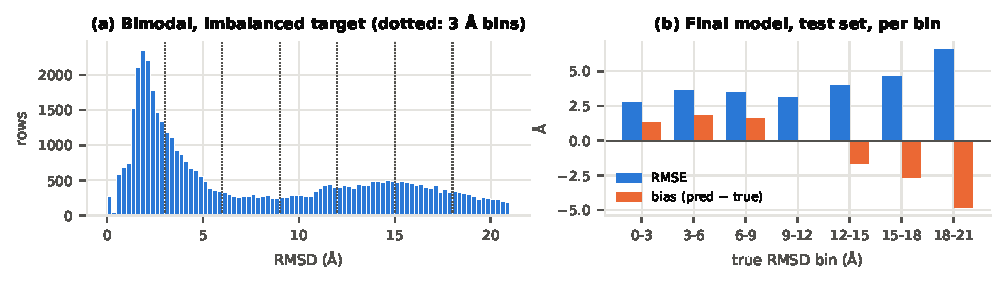
\includegraphics[width=\linewidth]{fig1_data.pdf}
  \caption{(a) The target is bimodal and imbalanced; the dotted lines are the 3\A{} bins. (b) The best Part~1 model
  (4$\times$256, ReLU, Adam $10^{-3}$, trained in notebook \S3.5) on the test set, per bin. Blue = RMSE in that bin.
  Orange = bias (prediction $-$ truth): positive means it guesses too high, negative means too low.}
  \label{fig:data}
\end{figure}

\subsection{Cleaning: duplicates}
\textbf{1{,}711 rows (3.7\%) were exact copies} (same features \emph{and} same target). We removed them
\textbf{before} splitting. If a row and its copy landed on opposite sides of the split, the model would be tested on a
row it had already memorised. That is leakage, and it makes the score optimistic.

A further 83 rows share identical features but have \emph{different} RMSD values. These were kept: they are genuine
noise in the labels, and no model can predict both values.

\subsection{Feature relevance}
\textbf{The question:} is any feature useless? We used three measures, each catching a different kind of relationship:

\begin{tabularx}{\linewidth}{@{}lYY@{}}
\toprule
Measure & What it detects & Weakness \\
\midrule
Pearson $r$ & A \textbf{straight-line} relationship ($-1$ to $+1$) & Misses curves. $r \approx 0$ does not mean ``no relationship'' \\
Spearman $\rho$ & A \textbf{consistently rising or falling} relationship (Pearson on the ranks) & Misses U-shapes \\
Mutual information (MI) & \textbf{Any} relationship: how much knowing the feature reduces uncertainty about the target & Has no fixed scale, so we added a \textbf{random-noise column} as the ``useless'' reference (MI = 0.000) \\
\bottomrule
\end{tabularx}

We also did a model-based check: gradient-boosted trees with 5-fold CV, leaving out one feature at a time to see how
much accuracy dropped.

\textbf{Findings.}
\begin{enumerate}
  \item \textbf{No feature is uninformative.} Every feature's MI (0.18--0.35) is far above the noise column's 0.000,
        even though five features have almost zero Pearson correlation. \textbf{F7 has $r = -0.003$ but the highest MI
        (0.350).} A correlation-only filter would have thrown away our most informative feature. The relationships are
        non-linear, which is also the argument for using an MLP instead of linear regression.
  \item \textbf{F2 is redundant: F2 = F1 $\times$ F3 exactly.} F3 is the \emph{fraction} of exposed area that is non-polar,
        so non-polar area (F2) = total area (F1) $\times$ that fraction. It adds no new information, so we dropped it.
  \item \textbf{F5 looked redundant but is not.} F5 $\approx 138.5 \times$ F1 (correlation 1.00), and the tree model barely
        noticed removing it. But the small deviation, the ratio F5/F1 (roughly the average mass of the exposed residues),
        carries information (MI 0.089). When we re-checked with \emph{the MLP itself} over 5 seeds, the model with F5
        beat the model without it in \textbf{5/5 seeds} (4.10 vs 4.15\A). So F5 was restored.
  \item Final decision: \textbf{8 inputs} (all except F2).
\end{enumerate}

\begin{keyidea}[Uninformative vs redundant (a likely test distinction)]
\textbf{Uninformative:} no relationship with the target at all (MI about the same as random noise). Remove it because it
only adds noise. \textbf{Redundant:} it is related to the target, but the same information is already in other features.
Removing it loses nothing. We found \emph{no} uninformative features and \emph{one} redundant one (F2).

\textbf{Lesson from F5:} ``redundant'' depends on the model. After the log transform, log F5 $-$ log F1 is a simple
difference that an MLP's first layer can compute with two weights, while a tree splits on one feature at a time and
struggles with differences. Always check feature decisions with the model you will actually use.
\end{keyidea}

\subsection{Outliers}
\textbf{Textbook rules.} The \textbf{IQR rule} flags a value as an outlier if it lies more than $1.5 \times$ IQR below the
25th percentile or above the 75th percentile (IQR = the spread of the middle 50\%). The \textbf{z-score rule} flags values
more than, say, 4 standard deviations from the mean. Both assume a roughly \emph{symmetric} distribution.

\textbf{The problem.} On right-skewed measurements such as areas, these rules mostly flag the \emph{natural long tail},
not errors. For example, the IQR rule flagged 1{,}864 F8 values. After a \texttt{log1p} transform, which squashes long
tails, those flags almost disappeared for F1, F4, F6 and F8. They were normal spread, not mistakes.

\textbf{F7 is the real exception.} Even after the log it has extreme values at both ends. But the rows with extreme F7
have ordinary RMSD values and ordinary other features. The anomaly is in F7 alone.

\textbf{Our strategy: transform and clip, don't delete.}
\begin{enumerate}
  \item \texttt{log1p(x)} = log(1 + x) on the skewed features. The ``+1'' is needed because F7 and F8 contain zeros.
  \item \textbf{Clip (winsorise)} every feature to its training-set \textbf{0.5th--99.5th percentile}. A value above the
        upper limit is replaced by the limit. The row is kept; only the extreme input value is capped, so it says
        ``very high'' instead of ``50 standard deviations high'' and cannot dominate a neuron's weighted sum.
\end{enumerate}

\textbf{Why not delete the rows?} (a) Their targets are valid and informative. (b) In real use we cannot refuse to
predict for a decoy with an odd F7, so the model must cope with such inputs anyway. (c) Deleting rows from the test
set would remove hard cases and flatter the score.

\textbf{The target is never treated as an outlier.} A large RMSD is a genuinely bad decoy, which is exactly what we
want to predict.

\subsection{Scaling}
Pipeline, fitted on training data: \textbf{select 8 features $\to$ log1p the skewed ones $\to$ clip $\to$ standardise.}

\textbf{Standardisation (z-score):} $z = (x - \mu) / \sigma$, using the training mean $\mu$ and standard deviation
$\sigma$. Afterwards every feature has mean 0 and standard deviation 1. Test data is transformed with the
\emph{same} training $\mu$ and $\sigma$.

\textbf{Why standardise at all?}
\begin{itemize}
  \item \textbf{One learning rate for all weights.} Raw F5 is around $10^6$ while F3 is around 0.3. Unscaled, the weights
        for different inputs would need learning rates that differ by orders of magnitude.
  \item \textbf{Initialisation assumptions.} Xavier and He initialisation assume inputs with roughly unit variance, so
        signals neither explode nor vanish as they pass through the layers.
  \item \textbf{Saturating activations.} Sigmoid and tanh go flat (gradient $\approx 0$) for large inputs. Standardised
        inputs start them in their responsive middle region.
\end{itemize}

\textbf{Why z-score rather than min-max (scaling to 0--1)?}
\begin{itemize}
  \item \textbf{Zero-centred.} Min-max values are all positive. If every input to a neuron is positive, all of its weight
        gradients share the same sign, so the weights can only all go up or all go down together, which causes
        zig-zagging and slow training.
  \item \textbf{Robust to extremes.} Min-max depends on the single largest and smallest value. F7's maximum would squeeze
        99\% of its values into a tiny slice of [0, 1].
\end{itemize}

\textbf{The target} is standardised for training too, so the loss is on a unit scale. Predictions are converted back
to ångström before \emph{any} metric is computed.

\subsection{Splitting, stratification and k-fold cross-validation}

\subsubsection*{Stratification}
\textbf{Stratification means every part of a split gets the same mix as the whole.} With classes (e.g.\ 10\% spam) it
guarantees each part is about 10\% spam. Our target is a number, not a class, so we \textbf{bin it temporarily} into
seven 3\A{} buckets (0--3, 3--6, \ldots, 18--21) and stratify on those bucket labels. The model still predicts the
actual number. Train and test bin shares then match to within 0.01 percentage points. Without stratification, a test
set or fold could by bad luck get too few of the rare high-RMSD decoys, and its score would be misleading.

\subsubsection*{k-fold cross-validation}
\textbf{The problem it solves:} to compare settings (Adam vs SGD, 2 vs 4 layers) we need a score on unseen data. We
cannot use the test set, because choosing by test score means the test set stops being a fair final exam. One single
validation chunk is fragile: the result depends on which rows happen to land in it.

\textbf{The idea:} cut the training data into $k$ equal folds. Run $k$ rounds. In each round one fold is held out for
scoring and the model trains on the other $k-1$. Every row is scored exactly once. Report the \textbf{mean $\pm$
standard deviation} of the $k$ scores.

\begin{center}
\small
\begin{tabular}{@{}lll@{}}
\toprule
Round & Train on rows & Score on rows \\
\midrule
1 & 3--10 & 1, 2 \\
2 & 1--2, 5--10 & 3, 4 \\
3 & 1--4, 7--10 & 5, 6 \\
4 & 1--6, 9--10 & 7, 8 \\
5 & 1--8 & 9, 10 \\
\bottomrule
\end{tabular}
\quad
\begin{minipage}{0.45\linewidth}
Example: 10 rows, $k = 5$. Scores 4.05, 4.12, 4.08, 4.15, 4.10 give \textbf{4.10 $\pm$ 0.04}. If another setting scores
4.11 $\pm$ 0.04, the difference is far smaller than the noise, so neither is better.
\end{minipage}
\end{center}

\textbf{Why it helps:} less luck (5 scores instead of 1); the standard deviation shows the noise level; no data wasted;
and the test set stays untouched. We used $k = 5$, and \textbf{every configuration saw exactly the same folds}, so
differences come from the configuration and not from easier folds. $k = 5$ is a standard trade-off: larger $k$ gives
more training data per round but costs $k$ trainings per configuration.

\textbf{Common misconception:} $k = 5$ is \emph{not} linked to the 80/20 split, and no fold is the test set. The test set
is removed first and never takes part in cross-validation.

\subsubsection*{The early-stopping split inside each fold}
Early stopping watches the error on separate data after each epoch and keeps the best epoch (Section~\ref{sec:es}).
That ``separate data'' must not be the fold we report, or we would be choosing the stopping epoch with the very data we
score, which is optimistic. So each round splits three ways:

\begin{center}
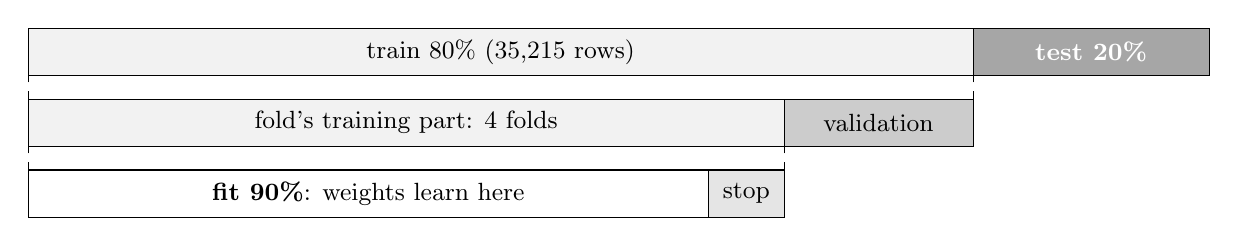
\begin{tikzpicture}[x=0.15cm,y=0.6cm,font=\small]
  % whole dataset
  \draw[fill=black!5] (0,3) rectangle (80,4); \node at (40,3.5) {train 80\% (35{,}215 rows)};
  \draw[fill=black!35] (80,3) rectangle (100,4); \node[white] at (90,3.5) {\textbf{test 20\%}};
  % one CV round on the training set
  \draw[fill=black!5] (0,1.5) rectangle (64,2.5); \node at (32,2) {fold's training part: 4 folds};
  \draw[fill=black!20] (64,1.5) rectangle (80,2.5); \node at (72,2) {validation};
  % inside the training part
  \draw[fill=white] (0,0) rectangle (57.6,1); \node at (28.8,0.5) {\textbf{fit 90\%}: weights learn here};
  \draw[fill=black!10] (57.6,0) rectangle (64,1); \node at (60.8,0.5) {stop};
  \draw[dashed] (0,2.5) -- (0,3); \draw[dashed] (80,2.5) -- (80,3);
  \draw[dashed] (0,1) -- (0,1.5); \draw[dashed] (64,1) -- (64,1.5);
\end{tikzpicture}
\end{center}
\begin{itemize}
  \item \textbf{Fit} ($\approx$25{,}300 rows): the weights learn here, and the preprocessing is fitted here.
  \item \textbf{Stop} ($\approx$2{,}800 rows): watched every epoch, only to decide when to stop.
  \item \textbf{Validation} ($\approx$7{,}000 rows): scored and reported, never used during training.
  \item \textbf{Test} (8{,}804 rows): locked until the very end.
\end{itemize}

\textbf{Limitation:} the data has no protein IDs. Many decoys come from the same protein and look alike, so
near-identical decoys can sit on both sides of a split. Absolute scores may therefore be slightly optimistic, but
\emph{comparisons} between settings are still fair, because every setting uses the same splits.

\subsection{Imbalance}
\textbf{For regression, ``imbalance'' means some ranges of the target are much rarer than others.} Our 0--3\A{} bin holds
34\% of rows, the 18--21\A{} bin only 7\% (4.9$\times$ fewer). A model trained with plain squared error is pulled
towards the common regions.

\begin{tabularx}{\linewidth}{@{}lY@{}}
\toprule
Stage & How we handle it \\
\midrule
Training & Stratified CV folds and stratified early-stopping split: every fold sees every RMSD range in the right proportion \\
Testing & The test split is stratified on the same bins, so the final score is a fair picture \\
Evaluation & Overall RMSE, MAE and $R^2$ \textbf{plus RMSE and bias per bin}, so failures in rare ranges cannot hide behind a good average \\
\bottomrule
\end{tabularx}

\textbf{Why per-bin reporting matters.} A model that always predicts the mean has an overall RMSE of 6.14\A, but per bin
its error ranges from 0.9\A{} (6--9\A, close to the mean) to 11.6\A{} (18--21\A). One number hides \emph{where} a model
fails. Our best model (Figure~\ref{fig:data}b) has 2.75\A{} error in the common 0--3\A{} bin but 6.56\A{} in the rare
18--21\A{} bin.

\textbf{Bias and regression to the mean.} Bias = average of (prediction $-$ truth) in a bin. Our model over-predicts the
good decoys (+1.3\A{} in 0--3\A) and under-predicts the bad ones ($-$4.8\A{} in 18--21\A). When unsure, it plays safe
and pulls its guesses towards the middle of the data.

\subsubsection*{Inverse-bin-frequency loss weights: tried and rejected}
\textbf{What it is:} each row's squared error is multiplied by 1 / (how common its bin is), so rows in rare bins count
more (a row in the 7\% bin weighs about 4.9$\times$ a row in the 34\% bin) and every bin contributes equally to the loss.
It is the regression version of \emph{class weights} in classification.

\textbf{Why we tried it:} it is the standard fix for imbalance, and the rare bins had the worst errors.

\textbf{Why we rejected it:}
\begin{enumerate}
  \item It moved errors around instead of removing them. Rare bins improved by 0.15--0.54\A, but the common 0--3\A{} bin
        got 1.02\A{} worse. \textbf{Overall RMSE rose from 4.09 to 4.31\A.}
  \item It did not fix the real problem. The under-prediction of bad decoys barely changed (bias $-$5.6 $\to$ $-$5.4\A);
        mostly it shifted \emph{all} predictions upwards. The model under-predicts bad decoys because the features cannot
        tell a very bad decoy from a moderately bad one, not because the loss ignores them. Re-weighting cannot add
        information that the features do not contain.
  \item The good, near-native decoys matter most in practice, and weighting made exactly those worse.
\end{enumerate}

\subsection{Measuring performance}
All metrics are computed in ångström, on data the model did not learn from.

\begin{tabularx}{\linewidth}{@{}lp{4.6cm}Y@{}}
\toprule
Metric & How it is calculated & What it means and why we use it \\
\midrule
\textbf{RMSE} & square root of the mean of $(\text{pred} - \text{true})^2$ & Typical error size, with big mistakes counting extra. Our headline metric: same units as the target, and it is the square root of MSE, which is exactly what the network is trained to minimise \\
\textbf{MAE} & mean of $|\text{pred} - \text{true}|$ & The plain average error. Always $\leq$ RMSE; a big gap means a few large errors \\
$\boldsymbol{R^2}$ & 1 $-$ (sum of our squared errors $\div$ sum of squared errors when always predicting the mean) & Fraction of the target's variation explained. 1 = perfect, 0 = no better than guessing the mean, $<0$ = worse. Gives a unit-free sense of ``good'' \\
\bottomrule
\end{tabularx}

\textbf{Worked example.} True values 2, 10, 18; predictions 4, 9, 12. Errors +2, $-$1, $-$6; squared 4, 1, 36.
RMSE = $\sqrt{41/3} \approx 3.70$. MAE = $9/3 = 3.0$. The mean of the truth is 10, and predicting 10 everywhere gives
squared errors 64 + 0 + 64 = 128, so $R^2 = 1 - 41/128 \approx 0.68$.

\textbf{CV score vs test score.} The \emph{CV score} is the average over the validation folds; it is measured on training
data and used to \emph{choose} between configurations, many times. The \emph{test score} is measured once, on the locked
test set, after all choices are made. Our best model: CV 3.81\A, test 3.78\A. They agree, which shows that comparing
many configurations with CV did not fool us (picking the best of many can pick a lucky one, which would make the test
score worse than the CV score).

\textbf{``Evaluation''} means \emph{how} we score: which metrics, on which data, broken down how. ``Testing'' is the data;
``evaluation'' is the measuring.

\begin{cheat}{Cheat sheet: data preparation}
\begin{itemize}
  \item \textbf{Leakage rule:} after the split, fit everything (MI, percentiles, $\mu$, $\sigma$) on training rows only.
  \item \textbf{Cleaning:} removed 1{,}711 exact duplicates \emph{before} splitting $\to$ 44{,}019 rows.
  \item \textbf{Relevance:} Pearson (linear), Spearman (monotonic), MI (any), plus a noise column and a tree
        leave-one-out check. None uninformative. \textbf{F2 = F1 $\times$ F3} dropped as redundant. F5 kept after an MLP check
        (5/5 seeds). F7: $r \approx 0$ but highest MI. 8 inputs.
  \item \textbf{Outliers:} IQR/z-score rules flag the natural tail of skewed data. log1p, then clip to the training
        0.5--99.5th percentile. No rows deleted. Target never clipped.
  \item \textbf{Scaling:} z-score (zero-centred, matches Xavier/He, keeps sigmoid/tanh responsive, robust to F7's extremes).
        Target standardised, metrics reported in \AA.
  \item \textbf{Splitting:} 80/20 stratified on 3\A{} bins (seed 42); 5-fold stratified CV on train; 10\% of each fold's
        training part for early stopping. Limitation: no protein IDs.
  \item \textbf{Imbalance:} 34\% vs 7\% bins. Stratified folds + stratified test + per-bin RMSE and bias. Loss weighting
        rejected (4.09 $\to$ 4.31\A; high-RMSD bias barely moved).
  \item \textbf{Metrics:} RMSE (headline), MAE, $R^2$. CV score chooses; test score reports, once.
\end{itemize}
\end{cheat}

\subsection{Likely questions: data preparation}

\Q{How did you decide whether a feature was uninformative? Why is correlation alone not enough?}
We compared each feature with the target using Pearson (linear), Spearman (monotonic) and mutual information (any
relationship), with a random-noise column as the ``useless'' reference, and checked with a model that left out one
feature at a time. Correlation only sees straight-line or monotonic patterns. F7 had $r = -0.003$ but the highest MI of
all features, so a correlation filter would have removed our most informative feature. No feature was uninformative.

\Q{Did you remove any features? Justify it.}
Only F2, because it is \emph{redundant}, not uninformative: F2 = F1 $\times$ F3 exactly, so it carries no new information
and adding it back changed nothing. F5 also looked redundant (F5 $\approx 138.5\times$F1), but the MLP was consistently
better with it (5/5 seeds), because the ratio F5/F1 carries information. Redundancy depends on the model.

\Q{How did you identify outliers, and how did you handle them? Why not just delete them?}
IQR and z-score counts, before and after a log transform. Most ``outliers'' were the natural tail of skewed
measurements and vanished after log1p; only F7 had genuine anomalies, and those rows had ordinary targets. We log-
transformed the skewed features and clipped every feature to its training 0.5th--99.5th percentile. Deleting would
throw away valid targets, would be impossible at prediction time, and would make the test set easier than reality.

\Q{Why should an outlier in the target not be removed?}
A large target value (a very bad decoy, a rare class, a high temperature) is real and is often exactly what we most
need to predict. Removing it teaches the model that such values do not exist and makes the evaluation dishonest.

\Q{Which scaling did you use and why, given your feature types?}
All features are continuous (F8 is a count with hundreds of levels), so one treatment fits all: log1p for skewed
features, clip, then z-score standardisation. Z-scores are zero-centred (avoids all of a neuron's gradients sharing one
sign), match the unit-variance assumption of Xavier/He initialisation, keep sigmoid/tanh out of their flat regions, and
unlike min-max they are not dominated by one extreme value. Categorical features would need one-hot encoding; we had none.

\Q{Why must the scaler be fitted on the training data only?}
To prevent data leakage. If test rows influenced the mean, standard deviation or clip limits, information about the
test set would be built into the model, and the test score would no longer be an honest estimate. It also mirrors real
use: future data is not available when you fit.

\Q{Describe your split strategy and justify it.}
80/20 train/test, stratified on 3\A{} RMSD bins with a fixed seed; the test set is used once at the end. All
comparisons use 5-fold stratified CV on the training set (the spec requires k-fold). Inside each fold, 10\% of the
training part is held out for early stopping. 20\% of 44k rows gives a precise test estimate, each validation fold still
has about 7k rows, and 5 folds keep the many experiments affordable.

\Q{What is k-fold cross-validation and why use it instead of a single validation set or the test set?}
See the k-fold section above. Short version: the training data is split into $k$ folds; each fold takes a turn as the
scored fold while the model trains on the rest; you report mean $\pm$ std. It gives a more reliable score than one split
(less luck), shows the noise level, uses all the data, and keeps the test set untouched so that it stays a fair final
exam.

\Q{Why stratify a split, and how can you stratify a regression target?}
So every part has the same target distribution, especially enough of the rare cases. For regression, bin the continuous
target into ranges and stratify on the bin labels.

\Q{Why is a separate early-stopping set needed inside each fold?}
Choosing the stopping epoch is a decision. Making it with the fold we report would let that fold influence the model,
so the reported score would be optimistic. A separate 10\% keeps ``choosing'' and ``scoring'' apart.

\Q{How did you handle imbalance during training, testing and evaluation?}
Training: stratified folds and early-stopping splits (and we tested inverse-frequency loss weights, which we rejected).
Testing: a stratified test split. Evaluation: per-bin RMSE and bias next to the overall metrics. For a classification
dataset the equivalents would be stratified splits, class weights or resampling, and per-class metrics such as precision,
recall and F1 instead of plain accuracy.

\Q{Why can a single overall metric be misleading on imbalanced data?}
It is dominated by the common cases. A model can look good overall while failing badly on the rare ones. In
classification, predicting ``not a pulsar'' for everything gives 91\% accuracy on HTRU2 and is useless. For us, overall
RMSE 3.78\A{} hides a 6.56\A{} error on the worst decoys.

\Q{Why did reweighting the loss not help?}
It traded accuracy on the common bins for accuracy on the rare bins (overall RMSE 4.09 $\to$ 4.31\A), and it did not fix
the under-prediction of bad decoys, because that comes from the features not separating those decoys, not from the loss
ignoring them.

\Q{Why remove duplicates before splitting rather than after?}
Once the split is made, copies are already on both sides; the model would be scored on rows it memorised (leakage).

\Q{Why might your test score still be optimistic?}
There are no protein IDs, so similar decoys of the same protein can appear in both train and test. We could not group
the split by protein. Comparisons between settings are unaffected because all settings use the same splits.

\newpage
% ================================================================ 2
\section{MLP building blocks (refresher)}
\label{sec:mlp}

\subsection{Our network}
Input (8) $\to$ [Linear $\to$ activation] repeated for each hidden layer $\to$ Linear $\to$ output (1 number).
\begin{itemize}
  \item The \textbf{output layer has no activation}, because this is regression and the output must be free to take any
        value (the standardised target is often negative). A sigmoid would cap it; a ReLU would forbid negatives.
  \item \textbf{Parameter count} of a layer = inputs $\times$ outputs + outputs (biases). The 2$\times$64 baseline:
        $(8\cdot64+64) + (64\cdot64+64) + (64\cdot1+1) = 4{,}801$. The 4$\times$256 network has about 200{,}000.
  \item Built in PyTorch, but the training loop, LR schedules, pruning masks and k-fold loop are written by hand in
        \texttt{src/}, so every step can be explained.
\end{itemize}

\subsection{One training step}
For every mini-batch of 256 rows (\texttt{src/training.py}):
\begin{enumerate}
  \item \textbf{Set the learning rate} for this step from the schedule. This is where warmup happens.
  \item \textbf{Forward pass:} each layer computes activation($Wx + b$), producing predictions.
  \item \textbf{Loss:} mean squared error between predictions and the true (standardised) targets.
  \item \textbf{Backward pass (backpropagation):} the chain rule, applied from the loss back through every layer, gives
        the gradient $\partial\text{loss}/\partial w$ for every weight. (Gradients are cleared first, because PyTorch adds
        new gradients to old ones.)
  \item \textbf{Update:} the optimiser moves every weight against its gradient. Plain SGD: $w \leftarrow w - \eta\, g$.
  \item (Part 2 only) re-apply the pruning masks so pruned weights stay at zero.
\end{enumerate}
One \textbf{epoch} = one pass over all training rows ($\approx$100 steps of 256 rows). The rows are reshuffled every
epoch. A \textbf{mini-batch} gradient is a noisy estimate of the full gradient; the noise is cheap and even helps escape
poor regions.

\subsection{Learning rate and schedules}
The \textbf{learning rate} $\eta$ is the size of each step. Too small: slow. Too large: the step overshoots the valley and
the loss can explode (\textbf{divergence}). A \textbf{schedule} changes $\eta$ during training:
\begin{itemize}
  \item \textbf{Constant:} the same $\eta$ throughout.
  \item \textbf{Cosine decay:} $\eta$ follows half a cosine wave from its peak down to 0. Large steps early for progress,
        small steps late so the weights settle into a minimum instead of bouncing around it.
  \item \textbf{Linear warmup:} $\eta$ rises in a straight line from nearly 0 to the peak over the first few epochs, then the
        normal schedule continues. Part 2 uses 5 epochs of warmup followed by cosine decay.
\end{itemize}

\subsection{Weight initialisation}
\textbf{Goal:} keep the size (variance) of the signals roughly the same from layer to layer, so they neither explode nor
vanish, in both the forward and the backward pass.
\begin{itemize}
  \item \textbf{Xavier / Glorot:} variance $2 / (\text{fan\_in} + \text{fan\_out})$. Designed for symmetric activations
        (sigmoid, tanh).
  \item \textbf{He / Kaiming:} variance $2 / \text{fan\_in}$, roughly twice Xavier's, because ReLU sets about half its
        inputs to zero and so halves the variance. Used with ReLU and its variants.
  \item \textbf{Naive random} (e.g.\ a fixed standard deviation of 0.01): ignores layer size, so in deep networks the
        signal shrinks layer after layer and training stalls.
  \item Biases start at 0, but weights must \textbf{not} all start equal: then every unit in a layer computes the same
        thing and gets the same update forever (no \textbf{symmetry breaking}).
\end{itemize}
We always matched the initialisation to the activation (``auto'': Xavier for sigmoid/tanh, He for ReLU).

\subsection{Overfitting and early stopping}
\label{sec:es}
\textbf{Overfitting:} the training error keeps falling, but the error on unseen data stops improving and eventually rises,
because the network starts memorising details of its training rows. Our baseline learning curves show it: training MSE
keeps dropping while the early-stopping MSE flattens after about 100 epochs.

\textbf{Early stopping} measures the error on the separate ``stop'' rows after every epoch, remembers the best epoch's
weights, and stops after 20 epochs without improvement (\textbf{patience} 20, because the curve is noisy). It then
\textbf{restores the best weights}, not the last ones. It is a form of \textbf{regularisation}: it limits how far the
network can overfit. (Maximum 500 epochs.)

\subsection{Regularisation in general (the axis we did not test)}
Regularisation = anything that stops a model from overfitting. The spec lists three:
\begin{itemize}
  \item \textbf{Weight decay (L2):} add $\lambda \sum w^2$ to the loss, so every step also shrinks the weights a little.
        Prefers simple, small-weight solutions. (It would interact with magnitude pruning, because it changes which weights
        are small.)
  \item \textbf{Dropout:} during training, randomly switch off a fraction of units at each step, so the network cannot rely
        on any single unit; like training many thinned networks at once. Switched off at evaluation.
  \item \textbf{Early stopping:} stop when the validation error stops improving (we used this).
\end{itemize}
\textbf{Expected behaviour:} without regularisation, a large network's training/validation gap grows; with it, the gap
shrinks, sometimes at a small cost in training fit. Too much regularisation causes underfitting.

\subsection{Baselines and noise}
\textbf{Why baselines?} ``RMSE 4.09\A'' means nothing on its own. Predict-the-mean (6.14\A, $R^2 = 0$) is the floor any
model must beat. Linear regression (5.19\A, $R^2 = 0.29$) tests whether non-linearity is needed (it is: the MLP is
$\sim$21\% better). Gradient-boosted trees (4.13\A) are a strong non-neural reference; matching them shows our MLP is
trained sensibly. All three are ready-made scikit-learn models, run through our own CV code with the same folds and
preprocessing (notebook \S2.2).

\textbf{Two kinds of noise:} \emph{fold-to-fold} (std 0.03--0.05\A, from which rows are in each fold) and
\emph{seed-to-seed} ($\sim$0.015\A, from the random initial weights and batch order). A \textbf{paired comparison} runs
both settings with the same seeds and folds and looks at the per-seed \emph{difference}, so shared noise cancels out.

\begin{cheat}{Cheat sheet: MLP building blocks}
\begin{itemize}
  \item Training step: set LR $\to$ forward $\to$ MSE loss $\to$ backprop $\to$ optimiser step (+ masks in Part 2).
  \item Output layer has no activation (regression). Parameters = in $\times$ out + out per layer.
  \item Xavier $2/(\text{in}+\text{out})$ for sigmoid/tanh; He $2/\text{in}$ for ReLU. Never all-equal weights.
  \item Early stopping: watch a separate split, keep the best epoch, patience 20. It is regularisation.
  \item Regularisation family: weight decay (shrink weights), dropout (random units off), early stopping.
  \item Schedules: constant, cosine decay, linear warmup then decay.
  \item Baselines: mean 6.14, linear 5.19, trees 4.13, MLP 2$\times$64 4.09\A.
  \item Noise: seed $\sim$0.015\A, fold std 0.03--0.05\A. Use paired comparisons.
\end{itemize}
\end{cheat}

\subsection{Likely questions: building blocks}

\Q{Walk through one training step of an MLP.}
Set this step's learning rate; forward pass to get predictions; compute the loss; zero the old gradients; backpropagate to
get every weight's gradient; let the optimiser update the weights.

\Q{Why compare against trivial baselines?}
They give the error a scale. Without them, nobody can tell whether 4.09\A{} is good. Predict-the-mean is the floor;
linear regression shows whether a non-linear model is needed.

\Q{What does early stopping monitor and why does it help?}
The error on a held-out split after each epoch. It keeps the best weights and stops once the error has not improved for
a while, which prevents the network from carrying on into overfitting.

\Q{Why pair Xavier with tanh/sigmoid and He with ReLU?}
Both keep the signal variance stable across layers. ReLU discards about half of its inputs, so He uses twice the
variance to compensate.

\Q{The training loss keeps falling but the validation loss flattens and rises. What is happening, and what can you do?}
Overfitting. Use early stopping, weight decay, dropout, more data, or a smaller network.

\Q{How do you know whether a difference between two settings is real?}
Compare it with the noise: fold-to-fold and seed-to-seed spread. We required a difference larger than that noise
\emph{and} in the same direction in every seed (a paired comparison).

\newpage
% ================================================================ 3
\section{Core investigation (the axes)}
\label{sec:core}

\subsection{What we did and how}
The spec asks for a baseline and controlled experiments on at least two of five axes (initialisation, activation
functions, architecture, optimisers, regularisation), evaluated with k-fold CV, with a hypothesis stated before each
one. We chose \textbf{three}:
\begin{itemize}
  \item \textbf{Optimisers}, because warmup in Part 2 is a learning-rate question, and optimisers decide how the LR acts.
  \item \textbf{Architecture}, to choose a principled network size, with enough spare capacity to prune.
  \item \textbf{Activation functions}, chosen instead of regularisation because they are easy to reason about, and they
        let us show vanishing gradients directly. Initialisation was always matched to the activation.
\end{itemize}

\textbf{Protocol for every axis.} Hypotheses written and committed before running. Change one thing; everything else stays
at the baseline (2$\times$64, ReLU, He, Adam $10^{-3}$, batch 256, early stopping). Each configuration: \textbf{3 seeds
$\times$ 5 folds}. Same four measurements on every axis:

\begin{tabularx}{\linewidth}{@{}lY@{}}
\toprule
Final quality & CV RMSE of the early-stopped model (mean over folds, averaged over seeds) \\
Convergence speed & Epochs until the early-stopping MSE first drops below \textbf{0.50} (standardised units: predicting the mean scores 1.0, the baseline ends at about 0.43) \\
Stability & Folds that diverged, and the spread across folds and seeds \\
Learning curves & Early-stopping MSE per epoch, to see \emph{how} configurations differ \\
\bottomrule
\end{tabularx}

\begin{keyidea}[The mistake that framed our hypotheses (worth mentioning)]
In the baseline phase, the MLP and gradient-boosted trees both stopped at $R^2 \approx 0.55$. We concluded that the
features set a ``ceiling'', and several hypotheses predicted only \emph{small} differences in final quality. The
architecture axis then showed a 4$\times$256 MLP reaching $R^2 = 0.615$. The ceiling was really the baseline's limited
capacity. Lesson: two models agreeing is weak evidence of a ceiling; test it by making the model bigger. Being wrong for
a clear, identifiable reason is a legitimate result.
\end{keyidea}

\subsection{Axis A: Optimisers}

\subsubsection*{The theory}
Notation: $w$ = a weight, $g$ = its gradient this step, $\eta$ = learning rate.

\begin{tabularx}{\linewidth}{@{}lp{5.3cm}Y@{}}
\toprule
Optimiser & Update & Idea \\
\midrule
SGD & $w \leftarrow w - \eta g$ & Step straight downhill \\
SGD + momentum & $v \leftarrow \beta v + g$; \; $w \leftarrow w - \eta v$ \; ($\beta = 0.9$) & Keep a running velocity: steady directions build up speed, zig-zags cancel out \\
RMSprop & $s \leftarrow \rho s + (1-\rho) g^2$; \; $w \leftarrow w - \eta g/(\sqrt{s}+\epsilon)$ & Divide each weight's step by its recent typical gradient size, so all weights take similar-sized steps \\
Adam & momentum average $m$ and squared average $s$, both bias-corrected; $w \leftarrow w - \eta \hat m / (\sqrt{\hat s}+\epsilon)$ & Momentum \textbf{plus} RMSprop-style scaling \\
\bottomrule
\end{tabularx}
\begin{itemize}
  \item \textbf{Momentum's effective step:} if the gradient stays similar, $v$ grows to $g / (1-\beta) = 10g$, so the step
        is about \textbf{10$\times$ the LR}. Momentum therefore blows up at a lower LR than plain SGD.
  \item \textbf{Adaptive methods} (RMSprop, Adam) make the step size roughly independent of the gradient's scale, which
        makes them forgiving of the LR choice and partly hides tiny (vanishing) gradients.
  \item \textbf{Bias correction (Adam only):} $m$ and $s$ start at 0, so early on they underestimate the true averages.
        Adam divides by $(1 - \beta^t)$ to fix this. PyTorch's RMSprop has \emph{no} bias correction.
\end{itemize}

\subsubsection*{Design}
All four optimisers on the \textbf{same LR grid} $\{10^{-4}, 3\cdot10^{-4}, 10^{-3}, 3\cdot10^{-3}, 10^{-2},
3\cdot10^{-2}, 10^{-1}\}$ $\times$ 3 seeds. One fixed LR would be unfair because each optimiser has its own natural LR
scale; the grid finds each one's best LR \emph{and} shows how sensitive it is to the choice.

\subsubsection*{Hypotheses, results and verdicts}
\begin{tabularx}{\linewidth}{@{}llrrr@{}}
\toprule
Optimiser & Best LR & CV RMSE & Epochs to 0.50 & Good LRs$^*$ \\
\midrule
Adam & $10^{-2}$ & \textbf{3.99} & \textbf{9.7} & 3 \\
SGD + momentum & $3\cdot10^{-2}$ & 4.03 & 12.5 & 2 \\
RMSprop & $3\cdot10^{-3}$ & 4.21 & 29.5 & 0 \\
SGD & $3\cdot10^{-3}$ & 4.39 & 293 (6/15 folds) & 0 \\
\bottomrule
\end{tabularx}
{\small $^*$ grid LRs giving a model within 0.10\A{} of the overall best.}

\textbf{H-A1 (speed): ``Adam and RMSprop fastest, plain SGD slowest, momentum in between.''} \verdict{Partly supported}
Adam was fastest and SGD slowest, as predicted. But \textbf{momentum beat RMSprop}: momentum alone gave about a 20$\times$
speed-up over plain SGD. \emph{Why we were partly wrong:} we assumed the adaptive scaling was the main source of speed. In
fact much of Adam's speed comes from the momentum it contains.

\textbf{H-A2 (final quality): ``At their best LRs, all four end within 0.05\A.''} \verdict{Contradicted}
The spread was 0.40\A. \emph{Why:} with a fixed budget (500 epochs) and early stopping, plain SGD never reached the good
region. At small LRs it hit the 500-epoch limit still improving; at larger LRs early stopping ended it early at a worse
score. \textbf{Under a limited budget, speed becomes final quality.} The hypothesis also relied on the false ``ceiling''.

\textbf{H-A3 (LR tolerance): ``Adam and RMSprop are good over a wider LR range than SGD; momentum diverges at a lower LR than
plain SGD.''} \verdict{Mixed}
Adam was the most tolerant (3 good LRs), as predicted. \textbf{RMSprop was the least tolerant}: it diverged in 11/15 folds at
$3\cdot10^{-2}$ and all folds at $10^{-1}$. The momentum part held: momentum broke at $10^{-1}$ while plain SGD still
trained there, consistent with its $\sim$10$\times$ effective step.
\emph{Why RMSprop failed (we measured it):} without bias correction, its squared-gradient average starts at 0, so its
\textbf{first update is 10$\times$ the LR}, while Adam's is exactly 1$\times$. Oversized steps at the very start of
training are exactly the problem \textbf{warmup} solves, which links this axis to Part 2.

\textbf{Side effect: dead units.} Large LRs knock ReLU units into permanently ``off'': Adam's dead fraction rose from 0.3\%
($10^{-3}$) to 10\%, 32\% and 48\% ($10^{-1}$).

\subsection{Axis B: Architecture (depth vs width)}

\subsubsection*{The theory}
\begin{itemize}
  \item \textbf{Width} = units per layer: how many features a layer computes side by side.
  \item \textbf{Depth} = number of layers: how many times features can be built \emph{from} other features (composition).
  \item \textbf{Universal approximation:} one hidden layer can approximate any continuous function given enough units, but
        depth can often do the same with far fewer units.
  \item \textbf{Costs:} depth makes the gradient path longer (risk of vanishing/exploding gradients, harder optimisation).
        Size in general means more capacity to memorise (overfitting) and slower training.
\end{itemize}

\subsubsection*{Design}
Depth $\{1,2,3,4\}$ $\times$ width $\{16, 64, 256\}$: 12 networks from 161 to $\sim$200k parameters, $\times$ 3 seeds,
baseline otherwise. Also recorded: parameter count, best epoch, and the train--validation gap at the kept epoch (an
overfitting indicator). Limitation: every size used the same LR ($10^{-3}$).

\subsubsection*{Results (CV RMSE in \AA, mean of 3 seeds; seed std $\leq$ 0.03)}
\begin{center}
\begin{tabular}{@{}lccc@{}}
\toprule
depth $\backslash$ width & 16 & 64 & 256 \\
\midrule
1 & 4.63 & 4.39 & 4.23 \\
2 & 4.42 & 4.09 (baseline) & 3.95 \\
3 & 4.33 & 4.00 & 3.83 \\
4 & 4.30 & 3.97 & \textbf{3.81} ($R^2$ 0.615) \\
\bottomrule
\end{tabular}
\end{center}

\textbf{H-B1 (width): ``16 $\to$ 64 clearly helps; 64 $\to$ 256 helps less than 0.05\A.''} \verdict{Partly supported}
16 $\to$ 64: $-0.33$\A; 64 $\to$ 256: $-0.14$\A. Returns do diminish, but the second gain is about 3$\times$ what we
predicted. \emph{Why wrong:} we assumed the feature ceiling; the baseline was capacity-limited.

\textbf{H-B2 (depth): ``2 layers beat 1; beyond 2, less than 0.05\A{} gain.''} \verdict{Half supported}
1 $\to$ 2 layers: $-0.30$\A, as predicted. But 2 $\to$ 3 ($-0.09$) and 2 $\to$ 4 ($-0.12$\A) still helped clearly.
\emph{Why wrong:} same ceiling assumption.

\textbf{H-B3 (overfitting): ``Bigger nets overfit sooner, but early stopping stops them ending worse.''}
\verdict{Supported} The kept epoch fell from $\sim$310 (1$\times$16) to $\sim$54 (4$\times$256), and the train--validation
gap rose from $\approx$0 to 0.19, so bigger nets overfit sooner and more. Early stopping caught them in time, and the
biggest net finished best.

\textbf{Extra findings:} depth was more parameter-efficient than width: 4$\times$64 (13k parameters) matched 2$\times$256
(68k) to within 0.014\A. Bigger nets also learned faster: 4$\times$256 reached MSE $<$ 0.50 in 5 epochs vs 21 for 2$\times$64.

\subsection{Axis C: Activation functions}

\subsubsection*{The theory}
\begin{tabularx}{\linewidth}{@{}lllY@{}}
\toprule
Activation & Formula & Max derivative & Notes \\
\midrule
Sigmoid & $1/(1+e^{-x})$ & \textbf{0.25} & Output (0, 1): not zero-centred. Saturates (flat) for large $|x|$ \\
tanh & $(e^x - e^{-x})/(e^x + e^{-x})$ & 1 & Output ($-1$, 1): zero-centred. Still saturates \\
ReLU & $\max(0, x)$ & 1 (0 if $x<0$) & No saturation for $x>0$, cheap. Units can ``die'' \\
Leaky ReLU & $x$ if $x>0$, else $0.01x$ & 1 (0.01 if $x<0$) & Never completely dead \\
\bottomrule
\end{tabularx}
\begin{itemize}
  \item \textbf{Vanishing gradients:} backprop multiplies by one activation derivative per layer. For sigmoid that factor
        is at most 0.25, so after $L$ layers the gradient reaching the first layer can shrink by up to $0.25^L$. Early layers
        then barely learn. ReLU's derivative is exactly 1 for active units, so gradients pass through undiminished.
  \item \textbf{Zero-centring:} sigmoid outputs are all positive, so the next layer's inputs are all positive and its weight
        gradients share one sign (zig-zag updates). tanh avoids this.
  \item \textbf{Dead ReLU:} if a unit's input is $\leq 0$ for every row (e.g.\ after a huge update), it outputs 0, gets zero
        gradient and can never recover. Leaky ReLU keeps a small slope so it can come back.
\end{itemize}

\subsubsection*{Design}
Sigmoid, tanh, ReLU and Leaky ReLU (with matching initialisation), at 2$\times$64 and a deeper 4$\times$64, $\times$ 3
seeds, Adam $10^{-3}$. Two diagnostics: (1) \textbf{gradient flow at initialisation}: the average gradient size in the first
layer divided by that in the last layer; far below 1 means vanishing gradients. (2) \textbf{dead units}: the fraction of
ReLU units that output 0 for every validation row.

\subsubsection*{Results}
\begin{center}
\small
\begin{tabular}{@{}lccc@{}}
\toprule
Activation & RMSE 2$\times$64 & RMSE 4$\times$64 & Epochs to 0.50 (2$\times$64 / 4$\times$64) \\
\midrule
Sigmoid & 4.34 & 4.26 & 423 / 340 \\
tanh & 4.06 & \textbf{3.90} & 64 / 21 \\
ReLU & 4.09 & 3.97 & 21 / 8.6 \\
Leaky ReLU & 4.10 & 3.96 & 21 / 8.5 \\
\bottomrule
\end{tabular}

\medskip
\textbf{Gradient flow at initialisation} (first layer's gradient size $\div$ last layer's; far below 1 = vanishing)\\[0.3em]
\begin{tabular}{@{}lccc@{}}
\toprule
First $\div$ last & depth 2 & depth 4 & depth 8 \\
\midrule
Sigmoid & 2.7e-3 & 1.7e-4 & \textbf{5.8e-7} \\
tanh & 0.31 & 0.27 & 0.33 \\
ReLU & 0.095 & 0.091 & 0.080 \\
\bottomrule
\end{tabular}
\end{center}

\textbf{H-C1 (speed): ``ReLU family fastest, then tanh, then sigmoid.''} \verdict{Supported}
8.6 / 21 / 340 epochs at 4$\times$64. Sigmoid's small derivative and non-zero-centred output make it slow.

\textbf{H-C2 (vanishing gradients): ``Sigmoid's gradient ratio is far smaller and shrinks with depth; its RMSE gap grows with
depth, but Adam softens the effect.''} \verdict{Supported}
With sigmoid the gradient shrinks by \textbf{about 4$\times$ per layer} going backwards, exactly what its maximum derivative
of 0.25 predicts; with 8 layers the first layer gets about a millionth of the output layer's gradient. tanh and ReLU stay
flat across depths. But in RMSE the sigmoid gap grew only slightly (0.25 $\to$ 0.30\A), and sigmoid even improved from
depth 2 to 4. \emph{Why:} Adam divides each weight's step by that weight's own gradient size, so tiny gradients still give
normal-sized steps. The damage showed up as \emph{slow} training, not failure. With plain SGD it would have been far worse.

\textbf{H-C3 (ReLU vs Leaky ReLU): ``tanh, ReLU and Leaky ReLU within 0.05\A; Leaky gains nothing because few ReLU units
die.''} \verdict{Partly supported}
Leaky ReLU = ReLU, and fewer than 0.5\% of ReLU units died, so the reasoning held: there was nothing for Leaky to fix.
But \textbf{tanh beat ReLU at depth 4} (3.90 vs 3.97\A, 3/3 seeds) while training 2.5$\times$ slower. A plausible but
untested reason: tanh networks are smooth, while ReLU networks are piecewise linear.

\subsection{The axes we did not run (in case they are asked)}
\textbf{Initialisation} (random vs Xavier/He). \emph{Hypothesis we would make:} a fixed small-random initialisation
(std 0.01) trains much more slowly, and fails in deeper nets, because the signal shrinks layer by layer; Xavier suits
tanh/sigmoid, He suits ReLU. \emph{How to test:} same network and optimiser, swap only the initialisation, compare
convergence speed and the gradient-flow ratio at several depths. Our code supports \texttt{init="random"}.

\textbf{Regularisation} (weight decay, dropout, early stopping). \emph{Hypothesis we would make:} on our large 4$\times$256
network, weight decay or dropout would reduce the train--validation gap and allow later stopping, with at most a small
gain in CV RMSE, because early stopping already controls overfitting well. \emph{How to test:} a grid of decay strengths
and dropout rates, measure the gap and the CV RMSE.

\subsection{Final test evaluation}
After all CV comparisons, the test set was used \textbf{once} (notebook \S3.5): the best CV-validated configuration
(4$\times$256, ReLU, Adam $10^{-3}$) and the baseline, each trained on the whole training set (90\% fit, 10\% stop) with
5 seeds. We deliberately did \emph{not} try untested combinations (such as Adam at $10^{-2}$ with 4$\times$256, or tanh),
because picking between them on the test set would be selecting on the test set.

\begin{center}
\small
\begin{tabular}{@{}lccc@{}}
\toprule
Model & CV RMSE & Test RMSE & Test $R^2$ \\
\midrule
Predict the mean & 6.14 & 6.14 & 0.00 \\
Linear regression & 5.19 & 5.19 & 0.29 \\
Baseline 2$\times$64 & 4.09 & 4.05 $\pm$ 0.04 & 0.566 \\
\textbf{Best 4$\times$256} & 3.81 & \textbf{3.78 $\pm$ 0.03} & \textbf{0.621} \\
\bottomrule
\end{tabular}
\end{center}
CV and test agree, so model selection did not overfit the validation folds. The bigger network helped most at the
extremes (0--3\A: 3.08 $\to$ 2.75\A; 18--21\A: 7.09 $\to$ 6.56\A), reducing but not removing the regression to the mean.

\subsection{Choosing the Part 2 network}
\begin{tabularx}{\linewidth}{@{}lY@{}}
\toprule
4$\times$256 & Best RMSE, and plenty of spare capacity for pruning to remove \\
ReLU, He & Fastest to train, and the standard in the pruning papers we follow \\
SGD + momentum 0.9 & It has a \textbf{sharp LR-tolerance boundary} (fine at $3\cdot10^{-2}$, broken at $10^{-1}$), which is exactly what the warmup question is about. Adam degrades gradually and self-corrects its early steps (bias correction), which would blur the effect. The original papers also used SGD with momentum \\
\bottomrule
\end{tabularx}

\begin{figure}[tbp]
  \centering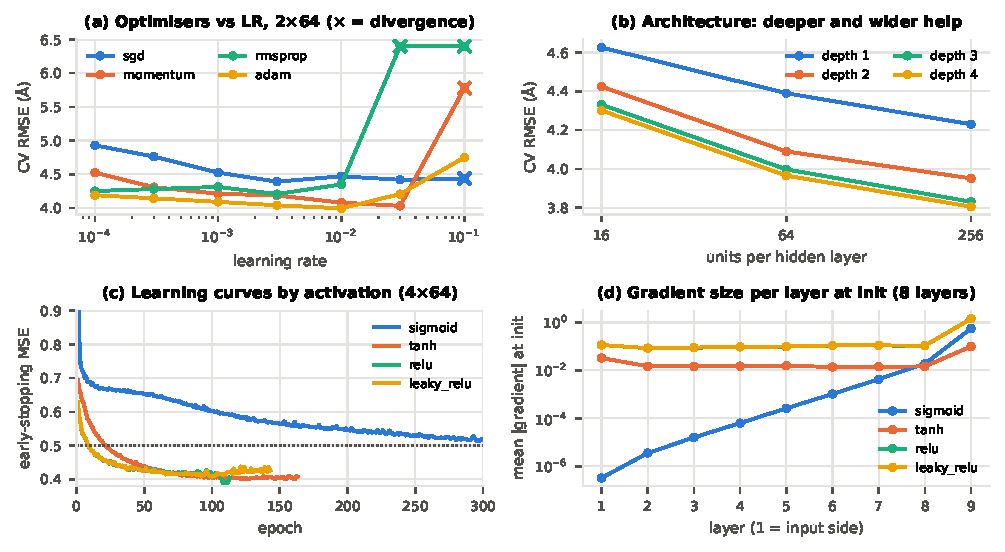
\includegraphics[width=\linewidth]{fig2_core.pdf}
  \caption{Core investigation. (a) Each optimiser across the LR grid ($\times$ = divergence). (b) RMSE by depth and width.
  (c) Learning curves by activation. (d) Gradient size per layer at initialisation, 8 hidden layers: sigmoid's collapses
  towards the input.}
\end{figure}

\begin{cheat}[unbreakable]{Cheat sheet: core investigation verdicts}
\small
\begin{tabularx}{\linewidth}{@{}p{5.6cm}lY@{}}
\toprule
Hypothesis & Verdict & Key evidence and reason \\
\midrule
A1 Adam/RMSprop fastest, SGD slowest & Partly & Adam 9.7, momentum 12.5, RMSprop 29.5, SGD 293 epochs. Momentum is the main speed source \\
A2 All optimisers end within 0.05\A & Contradicted & 3.99--4.39\A. Under a fixed budget, speed becomes quality \\
A3 Adaptive = LR-tolerant; momentum breaks before SGD & Mixed & Adam most tolerant; RMSprop least (no bias correction, first step 10$\times$ LR); momentum part true (10$\times$ effective step) \\
B1 Width: 64 $\to$ 256 adds $<$0.05\A & Partly & $-0.33$ then $-0.14$\A \\
B2 Depth: beyond 2 layers adds $<$0.05\A & Half & 1 $\to$ 2: $-0.30$; 2 $\to$ 4: $-0.12$\A \\
B3 Big nets overfit sooner; early stopping saves them & Supported & Best epoch 310 $\to$ 54; gap 0 $\to$ 0.19; 4$\times$256 best (3.81\A) \\
C1 Speed: ReLU $>$ tanh $>$ sigmoid & Supported & 8.6 / 21 / 340 epochs \\
C2 Sigmoid gradients vanish with depth; Adam softens it & Supported & $\approx$4$\times$ shrink per layer (0.25 derivative); shows in speed, not final RMSE \\
C3 tanh $\approx$ ReLU $\approx$ Leaky & Partly & Leaky = ReLU ($<$0.5\% dead); tanh beat ReLU at depth 4 \\
\bottomrule
\end{tabularx}
\textbf{Big lesson:} several hypotheses failed because of the false ``feature ceiling''; the baseline was capacity-limited.
Best model: 4$\times$256, CV 3.81\A, test 3.78\A, $R^2$ 0.621.
\end{cheat}

\subsection{Likely questions: core investigation}

\Q{Which axes did you investigate and why those?}
Optimisers (they control how the LR acts, which feeds the warmup question), architecture (to choose a principled
network size with capacity to prune) and activation functions (easy to reason about, and they show vanishing gradients).

\Q{State a hypothesis for one axis and say whether your results supported it.}
Use the template: e.g.\ H-C2: ``sigmoid's gradients shrink with depth because its derivative is at most 0.25.'' Design:
gradient ratio first/last layer at depths 2, 4, 8. Result: $\approx$4$\times$ shrink per layer, ratio 5.8e-7 at depth 8;
tanh and ReLU flat. Verdict: supported. Why: the chain rule multiplies one derivative per layer. Nuance: Adam hid most of
the effect in final RMSE.

\Q{Why did you compare optimisers on a grid of learning rates rather than at one learning rate?}
Each optimiser has its own natural LR scale (Adam around $10^{-3}$, SGD higher). At one LR you mostly measure which
optimiser that LR happens to suit. The grid compares each at its best LR and shows its sensitivity.

\Q{Explain how momentum speeds up SGD and why it can be less stable.}
It accumulates a velocity: directions the gradient keeps pointing in build up speed, and oscillating directions cancel.
With $\beta = 0.9$ the velocity reaches about 10$\times$ the gradient, so the effective step is about 10$\times$ the LR;
at a large LR that overshoots, which is why momentum diverged at $10^{-1}$ while plain SGD did not.

\Q{What does Adam adapt, and why is it forgiving of the learning rate?}
It keeps a momentum average and a squared-gradient average per weight and divides the step by the square root of the
latter. Step sizes become roughly independent of gradient scale, so a wide range of LRs works. Bias correction stops the
first steps from being oversized.

\Q{How did you measure convergence speed and stability?}
Speed: epochs until the early-stopping MSE first falls below 0.50. Stability: number of diverged folds and the spread
across folds and seeds.

\Q{Depth vs width: what does each give you, and which was better here?}
Width gives more features per layer; depth lets features be built from features. Depth costs longer gradient paths.
Here depth was more parameter-efficient (4$\times$64 with 13k parameters matched 2$\times$256 with 68k).

\Q{Bigger networks overfit more. Why was the biggest one best?}
Early stopping halted it at about epoch 54, before overfitting hurt the validation error. Capacity helps as long as
something controls the overfitting.

\Q{Why does sigmoid cause vanishing gradients, and why do tanh and ReLU help?}
Its derivative is at most 0.25 and near 0 when saturated; backprop multiplies these per layer, so gradients shrink
exponentially with depth. tanh's derivative reaches 1 and it is zero-centred; ReLU's derivative is exactly 1 for active
units.

\Q{What is a dead ReLU, and did it matter for you?}
A unit whose input is negative for every example outputs 0 and gets no gradient, so it never recovers. At normal LRs fewer
than 0.5\% died, so Leaky ReLU gave no benefit; at Adam LR $10^{-1}$, 48\% died.

\Q{One of your hypotheses was contradicted. Explain why.}
H-A2 (all optimisers end equal): under a fixed epoch budget and early stopping, the slow optimiser never reached the good
region, so speed turned into quality. Also it relied on a feature ceiling that turned out to be the baseline's capacity.

\Q{Why did you use only CV-validated configurations on the test set?}
Trying new combinations on the test set and keeping the best would make the test score optimistic. The CV and test
scores agreeing (3.81 vs 3.78\A) shows selection did not overfit.

\newpage
% ================================================================ 4
\section{Research investigation: warmup and pruning}
\label{sec:warmup}

\subsection{The question, in plain words}
The literature reports that a network trained with \textbf{learning-rate warmup} survives \textbf{pruning} better than
one trained without it, even when both are equally accurate before pruning. The proposed explanation is a two-link chain:
\begin{center}\small
\begin{tabular}{@{}ccccc@{}}
\textbf{warmup} & $\xrightarrow{\text{link 1, [3]}}$ & \textbf{a larger LR becomes trainable} & $\xrightarrow{\text{link 2, [2]}}$ & \textbf{better recovery from pruning} \\
\end{tabular}
\end{center}
So warmup might improve pruning robustness \emph{indirectly}. The spec stresses this is a hypothesis to test, not a fact.

\subsection{The three papers}
\begin{itemize}
  \item \textbf{[1] Frankle \& Carbin (2019), the Lottery Ticket Hypothesis.} A dense network contains a sparse subnetwork
        (a ``winning ticket'', often 10--20\% of the weights) that, trained from the \emph{same initial weights}, matches the
        full network. Found by iterative magnitude pruning. For deeper networks, warmup and a constant LR gave similar
        unpruned accuracy, but warmup gave much higher accuracy as the network was pruned further (Appendix I.5).
  \item \textbf{[2] Renda, Frankle \& Carbin (2020), rewinding vs fine-tuning.} Three ways to retrain after pruning:
        \textbf{fine-tuning} (continue from the final weights at a small fixed LR), \textbf{weight rewinding} (reset the
        surviving weights to an earlier point and retrain with the original schedule) and \textbf{LR rewinding} (keep the
        final weights, retrain with the original, large-LR schedule). Both rewinding methods beat fine-tuning, so a
        \emph{larger retraining LR helps recovery}.
  \item \textbf{[3] Kalra \& Barkeshli (2024), why warmup?} Warmup's main benefit is letting the network \textbf{tolerate a
        larger target LR}. At the start the loss surface can be sharp; small early steps move the network into a flatter,
        better-conditioned region, where large steps are safe.
\end{itemize}

\subsection{Key concepts}
\begin{itemize}
  \item \textbf{Warmup:} start with a tiny LR and raise it (here linearly over 5 epochs) to the target ``peak'' LR, then
        follow the normal schedule (here cosine decay to 0).
  \item \textbf{Pruning:} setting some weights to exactly zero to make the network smaller and faster.
        \textbf{Sparsity} = the fraction of weights removed (70\% sparsity keeps 30\%).
  \item \textbf{Magnitude pruning:} remove the weights with the smallest absolute value $|w|$, assuming they matter least.
  \item \textbf{Global vs layer-wise:} \emph{global} ranks all weights of all layers together, so layers can end up with
        different sparsities; \emph{layer-wise} removes the same fraction from every layer. We used \textbf{global}, and
        never pruned biases (few, and each shifts a whole unit).
  \item \textbf{One-shot vs iterative:} one-shot prunes to the target in one go; iterative prunes a little, retrains,
        repeats (as in [1]). We used \textbf{one-shot} (simpler, allowed by the spec, possibly a weaker effect).
  \item \textbf{Masks:} a 0/1 grid per weight matrix. During fine-tuning the masks are re-applied after every optimiser
        step, because the gradient and momentum would otherwise push pruned weights away from zero.
  \item \textbf{Robustness} = how much accuracy the network keeps when damaged by pruning. We measure it with $\Delta$.
\end{itemize}

\begin{keyidea}[$\Delta$: our robustness measure]
$\Delta(s)$ = test RMSE after pruning $s$\% and fine-tuning $-$ test RMSE of the unpruned network. Computed per seed,
then averaged. \textbf{Smaller $\Delta$ = more robust.} Using a difference removes the effect of slightly different
starting accuracies, so it isolates the damage done by pruning.
\end{keyidea}

\subsection{Fixed setup}
\begin{tabularx}{\linewidth}{@{}lY@{}}
\toprule
Network & 4$\times$256, ReLU, He ($\sim$200k weights) \\
Optimiser & SGD + momentum 0.9, batch 256 \\
Budget & \textbf{Fixed 100 epochs, no early stopping} (final weights kept), so every condition trains equally long \\
Schedule & Cosine decay to 0. Warmup conditions add 5 epochs of linear warmup first. \emph{The only difference is the warmup} \\
Data & Training set split once into fit 90\% / validation 10\%. \textbf{All choices on validation}; pruning results reported on the test set \\
Seeds & 3 for the LR sweep, \textbf{5} for the conditions (spec: $\geq 3$). Mean $\pm$ std \\
Pruning & One-shot global magnitude pruning at 0, 30, 50, 70, 90, 95, 98\% \\
Fine-tuning & \textbf{Identical for all}: SGD + momentum, constant LR 0.001, 10 epochs, masks re-applied \\
\bottomrule
\end{tabularx}

\subsection{Step 1: does warmup raise the tolerable learning rate? (H1)}
\textbf{H1:} ``The maximum stable LR with warmup is at least one grid step higher than without.''
\emph{Max stable LR} = the largest grid LR where all 3 seeds train without diverging and the validation RMSE is within
0.10\A{} of that schedule's best.

\textbf{Design:} train with and without warmup on the LR grid $\{0.005, 0.01, 0.02, 0.03, 0.05, 0.1, 0.2\}$ $\times$ 3
seeds; record validation RMSE and divergence.

\begin{center}
\small
\begin{tabular}{@{}lccccccc@{}}
\toprule
Peak LR & 0.005 & 0.01 & 0.02 & 0.03 & 0.05 & 0.1 & 0.2 \\
\midrule
No warmup (diverged seeds) & 3.73 (0) & 3.80 (\textbf{2/3}) & -- (3) & -- (3) & -- (3) & -- (3) & -- (3) \\
Warmup (diverged seeds) & 3.68 (0) & \textbf{3.63} (0) & 3.63 (0) & 3.66 (0) & 3.71 (0) & 3.71 (0) & 3.73 (0) \\
\bottomrule
\end{tabular}
\end{center}

\verdict{Strongly supported} Max stable LR \textbf{0.005 without warmup, 0.1 with warmup} (0.2 also trains but is a
hair outside the 0.10\A{} tolerance): \textbf{at least 20$\times$ higher}, 4 grid steps.
\textbf{All 17 no-warmup failures happened in the first epoch.} \emph{Why:} at initialisation the loss surface is sharp,
and full-size steps (amplified $\sim$10$\times$ by momentum) overshoot immediately. Warmup's small first steps move the
network to a calmer region before the big steps begin, exactly the mechanism in [3]. Warmup also gave better unpruned
models (3.63 vs 3.73\A).

\subsection{Step 2: choosing the conditions (rules fixed in advance)}
\begin{tabularx}{\linewidth}{@{}lY@{}}
\toprule
\textbf{A: no warmup, $\eta_0$} & $\eta_0$ = the no-warmup LR with the best validation RMSE $\to$ \textbf{0.005} \\
\textbf{B: warmup, $\eta_1 > \eta_0$} & The \emph{largest} warmup LR above $\eta_0$ that is stable and within \textbf{0.05\A} of A's validation RMSE (``comparable unpruned accuracy'') $\to$ \textbf{0.2} \\
\textbf{C: warmup, $\eta_0$ (control)} & Same LR as A, but with warmup $\to$ \textbf{0.005} \\
\bottomrule
\end{tabularx}

\textbf{Why ``comparable unpruned accuracy''?} The spec requires it, so that differences after pruning reflect robustness,
not a better starting point. Warmup LRs 0.01--0.03 were about 0.1\A{} \emph{better} than A, so they were not comparable;
LR 0.2 matched A (validation 3.73 vs 3.74\A{} over 5 seeds).

\textbf{Why the control C?} A and B differ in \emph{two} things at once: warmup \emph{and} learning rate. If B is more
robust, we could not tell which caused it. C has warmup but A's small LR, so it separates ``warmup itself'' from ``the
larger LR warmup allows''.

\textbf{Why fix the rules first?} Otherwise we could, even unintentionally, pick the B learning rate or the threshold that
makes the result look best. The rules were committed to git before running, so the conditions were chosen mechanically.

\subsection{Step 3: prune, fine-tune, compare (H2 and H3)}
For each condition $\times$ 5 seeds: train 100 epochs; then for each sparsity, prune a copy of the trained network,
measure test RMSE (``before fine-tuning''), fine-tune identically, measure again, and compute $\Delta$.

\textbf{H2:} ``At comparable unpruned RMSE, B (warmup, large LR) has a smaller $\Delta$ than A at high sparsity.''
\textbf{H3:} ``The benefit comes from the larger LR, not warmup itself: B beats C, while C $\approx$ A.''
\textbf{Counting rule (fixed in advance):} smaller $\Delta$ in $\geq$ 4/5 seeds (paired), by more than the standard
deviation of the paired differences, at $\geq$ 2 of the 4 sparsities $\geq$ 70\%.

\begin{center}
\small
\begin{tabular}{@{}l*{3}{>{\centering\arraybackslash}p{1.1cm}}@{\hspace{2.5em}}*{3}{>{\centering\arraybackslash}p{1.1cm}}@{}}
\toprule
& \multicolumn{3}{c}{Test RMSE \emph{before} fine-tuning (\AA)} & \multicolumn{3}{c}{$\Delta$ \emph{after} fine-tuning (\AA)} \\
Sparsity & A & B & C & A & B & C \\
\midrule
30\% & 4.35 & 3.89 & 4.60 & 0.03 & 0.00 & 0.03 \\
50\% & 5.69 & 4.08 & 6.15 & 0.08 & 0.02 & 0.11 \\
70\% & 7.97 & \textbf{4.61} & 7.39 & 0.31 & \textbf{0.09} & 0.35 \\
90\% & 8.59 & \textbf{5.86} & 7.82 & 0.71 & \textbf{0.44} & 0.74 \\
95\% & 7.51 & 6.40 & 7.15 & 0.95 & \textbf{0.69} & 1.01 \\
98\% & 6.74 & 6.45 & 6.69 & 1.34 & \textbf{1.09} & 1.40 \\
\bottomrule
\end{tabular}
\end{center}
Unpruned test RMSE: A 3.81, B 3.84, C 3.78\A{} (so B started slightly \emph{worse}).

\begin{tabularx}{\linewidth}{@{}lccY@{}}
\toprule
Comparison & Mean $\Delta$ difference & Seeds & Meets the rule? \\
\midrule
B vs A & $-0.22$ to $-0.27$\A & 5/5 at every sparsity & Yes, 4/4 sparsities $\to$ \textbf{H2 supported} \\
B vs C & $-0.26$ to $-0.32$\A & 5/5 at every sparsity & Yes, 4/4 \\
C vs A & $+0.03$ to $+0.06$\A{} (C slightly worse) & C better in 0--2/5 & No $\to$ with B vs C, \textbf{H3 supported} \\
\bottomrule
\end{tabularx}

\textbf{H2} \verdict{Supported} B lost 0.22--0.27\A{} less than A at every sparsity $\geq$ 70\%, in 5/5 seeds, about
5$\times$ the seed noise. \textbf{Before fine-tuning} the gap was dramatic: at 70\% sparsity B's error was 4.6\A{} while A and
C jumped to 8.0 and 7.4\A, \emph{worse than predicting the mean} (6.14\A). (A and C come back down at 98\% only because a
nearly empty network outputs almost a constant, which is close to the mean.)

\textbf{H3} \verdict{Supported} Warmup at the small LR (C) gave \emph{no} benefit over A, even though C had the best
unpruned RMSE. Only the large-LR network B was robust. So warmup helps pruning robustness \textbf{only through the larger
LR it makes possible}.

\subsection{Alternative explanations we ruled out (confounders)}
\begin{itemize}
  \item \textbf{Dead units as ``free'' sparsity.} Large LRs can kill ReLU units, and pruning a dead unit's weights costs
        nothing. But B had the \emph{fewest} dead units (A 3.6\%, B 0.2\%, C 0.0\%), so this cannot explain it.
  \item \textbf{Fine-tuning LR favouring B.} 0.001 is 20\% of A's and C's training LR but only 0.5\% of B's. By [2], a
        relatively larger retraining LR helps recovery, so this setup \emph{favours A and C}. B won anyway.
  \item \textbf{Starting point.} B's unpruned test RMSE was slightly worse than A's, so its advantage is not a head start.
  \item \textbf{Reference point.} Measuring $\Delta$ against the fine-tuned dense network instead gives the same ranking.
\end{itemize}

\textbf{Post-hoc look at the weights} (added after seeing the results, so exploration, not a test): A and C have almost
identical weight distributions, matching their identical pruning behaviour. B's weights are larger (median $|w|$ 0.084
vs 0.062) and more of its ``weight mass'' sits in its largest weights (top 10\% hold 60.6\% of $\sum w^2$ vs 56.5\%). A
network that relies more on a few large weights loses less when the many small ones are removed. Another untested
explanation: large-LR training ends in flatter minima, where zeroing weights changes the loss less.

\subsection{Extensions E1, E2, E3}
\begin{tabularx}{\linewidth}{@{}lYl@{}}
\toprule
& Question & Planned in advance? \\
\midrule
E1 & Does retraining with each network's own schedule (LR rewinding, from [2]) change the picture? & Yes \\
E2 & Does a longer warmup give more robustness (spec's ``warmup duration'' extension)? & Yes \\
E3 & Does robustness rise steadily with the LR among warmup networks (dose--response)? & \textbf{No, exploratory} \\
\bottomrule
\end{tabularx}

\textbf{E1: LR rewinding.} After pruning, retrain for 10 epochs with the network's \emph{own} schedule squeezed into 10
epochs (same peak LR, warmup for 5\% if it had one, cosine to 0), instead of the small fixed LR. $\Delta$ is measured
against each network's own retrained dense version, because rewinding improves the unpruned networks too (B 3.84 $\to$
3.72\A).
\emph{Prediction:} everyone recovers better, and the A--B gap shrinks. \emph{Result:} everyone recovered better, but the
gap \textbf{widened} (at 90\%: A 0.58\A, B 0.03\A). \verdict{Gap prediction contradicted}
\emph{Why:} B now retrains at LR 0.2 while A retrains at 0.005, and a large retraining LR recovers better ([2]). So the
large LR that warmup unlocks helps \textbf{twice}: more robust trained weights \emph{and} more effective recovery.

\textbf{E2: warmup duration} (condition B at LR 0.2 with 1, 5 or 15 warmup epochs).
\emph{Prediction:} once warmup makes LR 0.2 trainable, longer warmup adds nothing (a threshold effect).
\emph{Result:} even \textbf{1 epoch} made LR 0.2 trainable; 1 vs 5 epochs: no consistent difference; but \textbf{15 epochs
was less robust} than 5 (4--5/5 seeds, 0.04--0.12\A) while having the best unpruned RMSE (3.79\A).
\verdict{Partly supported} A plausible, untested reason: a longer warmup leaves fewer epochs at the large LR, and the
large LR is what creates robustness.

\textbf{E3: LR dose--response} (all 7 warmup LRs, 5 seeds each). ``Dose--response'' is a term from medicine: if more
dose gives steadily more effect, that is strong evidence of cause.
\begin{center}
\small
\begin{tabular}{@{}lccccccc@{}}
\toprule
Warmup LR & 0.005 & 0.01 & 0.02 & 0.03 & 0.05 & 0.1 & 0.2 \\
\midrule
Unpruned test RMSE & 3.78 & \textbf{3.76} & 3.79 & 3.82 & 3.84 & 3.84 & 3.84 \\
$\Delta$ at 70\% & 0.35 & 0.26 & 0.19 & 0.14 & \textbf{0.09} & 0.12 & \textbf{0.09} \\
$\Delta$ at 90\% & 0.74 & 0.65 & 0.54 & 0.51 & 0.49 & 0.51 & \textbf{0.44} \\
\bottomrule
\end{tabular}
\end{center}
Robustness rises steadily with the LR (Spearman correlation between LR and $\Delta$: $-0.88$ at 70\%). Crucially,
\textbf{LR 0.01 gave the best unpruned model but was far less robust than 0.2}, so robustness follows the LR, not the
starting accuracy. This strengthens H3 beyond the two-point comparison, but because it was designed after seeing the
results it counts as supporting evidence, not a formal test.

\begin{figure}[H]
  \centering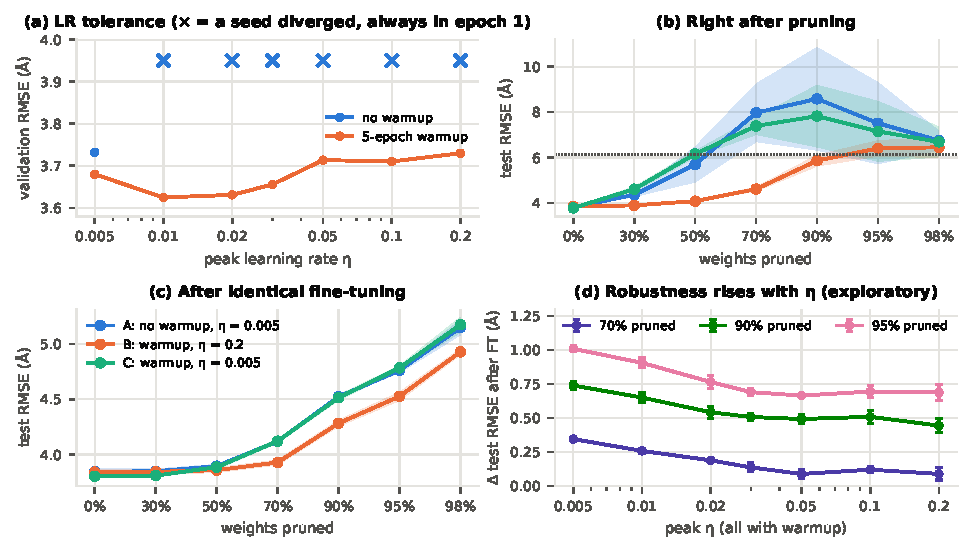
\includegraphics[width=\linewidth]{fig3_warmup_pruning.pdf}
  \caption{(a) LR tolerance: without warmup everything above 0.005 fails ($\times$). (b, c) Test RMSE vs sparsity for A, B,
  C before and after identical fine-tuning (the spec's ``accuracy vs sparsity'' plot; lower is better; dotted = predicting
  the mean). (d) E3: $\Delta$ falls as the warmup LR rises.}
\end{figure}

\subsection{Conclusion and limitations}
\textbf{Did we observe the effect?} Yes. At matched unpruned accuracy, the warmup-trained network lost 0.22--0.27\A{} less
after pruning and fine-tuning (5/5 seeds), and far less before fine-tuning.

\textbf{Do the results support the mechanism?} Yes, on both links. Link 1: warmup raised the tolerable LR $\geq$20$\times$
(H1). Link 2: the robustness comes from the larger LR, not from warmup itself (H3, with E3 showing a steady trend). E1
adds that the large LR also helps recovery. Warmup's effect is therefore \textbf{indirect}.

\textbf{Limitations:} one tabular dataset and one MLP (the papers used CNNs on images); one-shot rather than iterative
pruning; a single fit/validation split (seeds capture initialisation noise, not data-split noise); B's LR sits at the top
of the grid; large-LR training \emph{without} warmup cannot be tested because it diverges; and the reason large-LR
networks are robust is only explored post-hoc.

\subsection{The spec's other extensions (not done, but could be asked)}
\begin{itemize}
  \item \textbf{Timing} (prune during warmup vs well after it). \emph{Expectation:} during warmup the network has barely
        trained, so weight magnitudes say little about importance; pruning well after warmup should be better. \emph{Test:}
        prune at several epochs (e.g.\ 2, 5, 20, 100), same retraining budget, compare $\Delta$.
  \item \textbf{Distillation.} A small ``student'' network is trained to copy a large ``teacher's'' outputs. Question:
        does a warmup-trained teacher give a better student? \emph{Test:} train teachers with and without warmup at
        matched accuracy, distil identical students, compare.
  \item \textbf{Neural architecture search (NAS).} Automatically searching over architectures (e.g.\ random search).
        Question: does the schedule used to \emph{score} candidates during the search change which architecture wins, even
        if all are later retrained the same way? \emph{Test:} run the same search twice, with and without warmup, compare
        the selected architectures after full retraining.
\end{itemize}

\begin{cheat}{Cheat sheet: warmup and pruning}
\begin{itemize}
  \item \textbf{Chain:} warmup $\to$ larger trainable LR [3] $\to$ better pruning recovery [2]. Spec: test it.
  \item \textbf{Setup:} 4$\times$256 ReLU, momentum 0.9, 100 epochs, cosine; warmup = 5 linear epochs. 5 seeds.
  \item \textbf{H1} supported: max stable LR 0.005 (no warmup) vs 0.1, trains at 0.2 ($\geq$20$\times$). All failures in epoch 1.
  \item \textbf{Conditions} (rules fixed in advance): A no warmup 0.005; B warmup 0.2 (matched within 0.05\A); C warmup 0.005 (control).
  \item \textbf{Pruning:} one-shot global magnitude, biases kept, 0--98\%. \textbf{Fine-tune:} identical, LR 0.001, 10 epochs, masks.
  \item $\boldsymbol{\Delta}$ = RMSE after fine-tune $-$ unpruned RMSE. Smaller = more robust.
  \item \textbf{H2} supported: B's $\Delta$ 0.22--0.27\A{} smaller than A's at $\geq$70\%, 5/5 seeds. Before FT at 70\%: B 4.6 vs A 8.0\A.
  \item \textbf{H3} supported: C $\approx$ A (slightly worse); B beats C by 0.26--0.32\A. The LR is the cause.
  \item \textbf{Confounders ruled out:} dead units (B fewest), fine-tune LR (favours A/C), starting point (B slightly worse).
  \item \textbf{E1} LR rewinding: all recover better, A--B gap \emph{widens} (contradicted). Large LR helps twice.
  \item \textbf{E2} warmup length: 1 $\approx$ 5 epochs; 15 less robust (partly supported).
  \item \textbf{E3} (exploratory): $\Delta_{70\%}$ 0.35 $\to$ 0.09 as LR 0.005 $\to$ 0.2; Spearman $-0.88$.
  \item \textbf{Answer:} warmup improves pruning robustness \emph{indirectly}, by unlocking a large LR.
\end{itemize}
\end{cheat}

\subsection{Likely questions: warmup and pruning}

\Q{What is learning-rate warmup and why does it help?}
Start with a very small LR and increase it to the target over the first steps or epochs. According to Kalra \&
Barkeshli, its main benefit is that the network tolerates a larger target LR: the small early steps move it from a sharp,
unstable region into a flatter one before the large steps begin.

\Q{What is magnitude pruning? Global vs layer-wise? One-shot vs iterative?}
Remove the weights with the smallest absolute values. Global ranks all weights together; layer-wise removes the same
fraction from each layer. One-shot prunes once to the target sparsity; iterative prunes in small rounds with retraining
in between. We used one-shot global pruning of the weight matrices.

\Q{Why must the unpruned networks have comparable accuracy?}
So that any difference after pruning reflects robustness and not a better starting point. We required B's validation
RMSE to be within 0.05\A{} of A's, by a rule fixed in advance.

\Q{Why must the fine-tuning procedure be identical for both networks?}
Otherwise a difference after fine-tuning could come from the fine-tuning recipe rather than from how the networks were
trained. Same optimiser, LR, epochs and masks for all.

\Q{How did you separate the effect of warmup from the effect of a larger learning rate?}
With the control C: warmup at A's small LR. C behaved like A, while B (warmup with a large LR) was much more robust, so the
large LR is the cause and warmup is only the enabler.

\Q{Why did all no-warmup failures happen in the first epoch?}
At initialisation the loss surface is sharp; full-size steps, amplified about 10$\times$ by momentum, overshoot
immediately and the loss explodes. Warmup's small first steps avoid exactly that moment.

\Q{Why do pruning masks need to be re-applied after every step?}
A pruned weight still receives a gradient (and momentum), so one optimiser step would make it non-zero again. Multiplying
by the mask keeps the network truly sparse.

\Q{Why measure the error both before and after fine-tuning?}
Before shows the raw damage of removing weights; after shows how well the network recovers. The spec asks for the
recovered accuracy; B was better on both.

\Q{Why use at least three seeds and report mean $\pm$ std?}
One run can be lucky. Several seeds show how much results vary from initialisation and batch order, and paired
comparisons per seed let us check that a difference is consistent and larger than the noise.

\Q{What is fine-tuning vs learning-rate rewinding, and what did you find?}
Fine-tuning retrains the pruned network at a small fixed LR; LR rewinding retrains it with its original, large-LR
schedule. Rewinding improved recovery for all networks and widened B's advantage, because B rewinds to LR 0.2.

\Q{What is the Lottery Ticket Hypothesis?}
A large network contains a small subnetwork that, trained from the same initial weights, can match the full network's
accuracy. It is found with iterative magnitude pruning; for deeper networks, warmup helped find such subnetworks.

\Q{How do you read an accuracy-vs-sparsity plot?}
x-axis: fraction of weights removed; y-axis: error (for us, lower is better) or accuracy (higher is better). A robust
network's curve stays flat for longer before it rises. Compare curves at matched starting points, look at the gap at high
sparsity, and check the shaded spread across seeds.

\Q{Did your results support or contradict the proposed mechanism? What if they had contradicted it?}
They supported it on both links (H1, H3, E3). If they had contradicted it, possible reasons would be: a small,
over-parameterised MLP on tabular data is very different from the image CNNs in the papers; one-shot instead of iterative
pruning; or the network being so redundant that pruning barely hurts any condition. An honest ``contradicted'' is a
valid result.

\Q{What are the main threats to validity in your experiment?}
Comparability of unpruned accuracy, dead units acting as free sparsity, the fine-tuning LR being a choice, one-shot
pruning, a single fit/validation split, and only one dataset and architecture.

\newpage
% ================================================================ 5
\section{General research-method questions}
\label{sec:generic}
These apply to any of the five datasets and are the most likely kind of test question.

\Q{What makes a good hypothesis?}
It is stated \emph{before} the experiment, makes a specific, measurable prediction (``at least one grid step higher'',
``within 0.05\A''), gives a reason based on theory, and says what result would contradict it.

\Q{What makes an experiment controlled and fair?}
Change one variable at a time; keep everything else fixed; use the same data splits for every setting; repeat over
several seeds; decide the measurements and decision rules in advance; and include a control when two factors are tangled
together (our condition C).

\Q{Why should hypotheses and decision rules be written before running?}
So the result cannot shape the prediction. Otherwise it is easy, even unintentionally, to choose thresholds or settings
that make the outcome look good. We committed ours to git before running.

\Q{Your hypothesis was contradicted. Is the experiment a failure?}
No. A contradicted hypothesis is a real finding if the experiment was fair. Explain \emph{why} the reasoning was wrong: our
``feature ceiling'' assumption made several Part~1 hypotheses too pessimistic about capacity, and the architecture axis
revealed it.

\Q{Why not tune hyperparameters on the test set?}
The test set must be a fair, unseen final exam. Choosing settings by test score lets the test set influence the model,
so its score becomes optimistic and no longer estimates real-world performance.

\Q{How do you decide whether a difference is meaningful?}
Compare it with the noise (standard deviation across folds and seeds), and check that it points the same way in every
paired seed. A gap smaller than the noise is not evidence.

\Q{What is the difference between correlation and causation in your study?}
B being both large-LR and robust is a correlation. The control C (warmup without the large LR) and the dose--response
(E3) were needed to argue that the LR \emph{causes} the robustness.

\Q{How would you interpret a learning curve?}
Training and validation loss per epoch. Both falling: still learning. Training falling, validation flat or rising:
overfitting. Both high and flat: underfitting (too little capacity or too small an LR). Jagged: noisy updates, e.g.\ a
constant LR with small batches. Explodes: LR too large.

\Q{Why is reproducibility important, and how did you achieve it?}
Others (and you) must be able to repeat the result. Fixed seeds for splits, initialisation and batch order; results cached
to CSV; all code in the notebook and \texttt{src/}; pinned package versions.

\Q{What would you do differently or next?}
Group the split by protein if IDs were available; iterative pruning; k-fold instead of a single split in Part 2; test the
mechanism behind large-LR robustness (flatness, weight concentration) directly; try the regularisation and initialisation
axes.

\Q{How would your answers change for a classification dataset?}
Stratify directly on the class labels; handle imbalance with class weights or resampling; evaluate with per-class
precision, recall, F1 or AUC instead of plain accuracy; use cross-entropy loss with a sigmoid or softmax output.

\newpage
% ================================================================ 6
\section{Glossary}
\label{sec:glossary}
\small
\begin{xltabular}{\linewidth}{@{}>{\raggedright\arraybackslash}p{4.2cm}Y@{}}
\toprule
Term & Meaning \\
\midrule
\endhead
\AA{} (ångström) & $10^{-10}$ m. Unit of RMSD and of all our errors \\
Activation function & The non-linear function applied after each layer's weighted sum (sigmoid, tanh, ReLU) \\
Adam & Optimiser combining momentum with per-weight step scaling, plus bias correction \\
Backpropagation & Using the chain rule to compute every weight's gradient, from the loss backwards \\
Batch / mini-batch & The subset of rows (256) used for one gradient step \\
Bias (metric) & Mean of (prediction $-$ truth) in a group; positive = guesses too high \\
Bias correction & Adam's fix for its averages starting at 0 \\
Bimodal & A distribution with two peaks \\
Confounder & A hidden factor that could explain a result instead of the one you are testing \\
Control condition & A condition that isolates one factor (our C: warmup without the large LR) \\
Cosine decay & LR schedule following half a cosine wave from peak to 0 \\
Cross-validation (k-fold) & Rotate which fold is scored; average the $k$ scores \\
Data leakage & Information from evaluation data reaching the model during training or preprocessing \\
Dead ReLU & A unit that outputs 0 for every input and never recovers \\
Decoy & A candidate (predicted) 3D shape of a protein; one row of our data \\
Divergence & Training blowing up (loss becomes huge or NaN), usually from too large an LR \\
Dose--response & Effect growing steadily with the size of the cause; evidence of causation \\
Dropout & Randomly switching units off during training as regularisation \\
Early stopping & Stop when validation error stops improving; keep the best weights \\
Epoch & One pass over all training rows \\
Fine-tuning & Retraining a pruned network at a small fixed LR \\
Global pruning & Ranking all layers' weights together when pruning \\
He / Xavier init & Weight initialisations sized for ReLU / for sigmoid and tanh \\
IQR rule & Outlier if beyond 1.5 $\times$ IQR outside the 25th--75th percentiles \\
Learning rate (LR, $\eta$) & Size of each optimiser step \\
Lottery Ticket Hypothesis & Large nets contain small subnetworks that train to full accuracy from the same initial weights \\
LR rewinding & Retraining a pruned network with its original LR schedule \\
Magnitude pruning & Removing the weights with the smallest $|w|$ \\
MAE / RMSE / $R^2$ & Mean absolute error / root mean squared error / fraction of variance explained \\
Mask & 0/1 grid marking which weights are pruned \\
Momentum & Running velocity of gradients; effective step $\approx \eta/(1-\beta)$ \\
Mutual information & Measures any (incl.\ non-linear) dependence between two variables \\
Overfitting & Fitting training data so closely that performance on unseen data gets worse \\
Paired comparison & Comparing two settings seed-by-seed on the same folds so shared noise cancels \\
Pre-registration & Writing hypotheses and rules down before running the experiment \\
Redundant feature & Informative, but its information is already in other features \\
Regression to the mean & Predictions pulled towards the average: low values over-, high values under-predicted \\
RMSD & The target: how far a decoy's atoms are from the true structure (\AA) \\
RMSprop & Optimiser scaling each step by the recent gradient size (no bias correction in PyTorch) \\
Robustness ($\Delta$) & Extra error after pruning and fine-tuning; smaller is more robust \\
Saturation & Sigmoid/tanh going flat for large inputs, so the gradient $\approx 0$ \\
Seed & Number fixing the randomness (initial weights, batch order) \\
Sparsity & Fraction of weights set to zero \\
Stratification & Making every split have the same target (or class) mix as the whole \\
Uninformative feature & No relationship with the target \\
Vanishing gradients & Gradients shrinking layer by layer going backwards, so early layers barely learn \\
Warmup & Ramping the LR up from near 0 to its peak at the start of training \\
Weight decay & Penalty on large weights (L2) as regularisation \\
Winsorise (clip) & Replace values beyond a limit by the limit; the row is kept \\
Z-score & $(x-\mu)/\sigma$: standardisation to mean 0, std 1 \\
\bottomrule
\end{xltabular}

\end{document}
